\documentclass{VUMIFPSkursinis}
\usepackage{algorithmicx}
\usepackage{algorithm}
\usepackage{algpseudocode}
\usepackage{amsfonts}
\usepackage{amsmath}
\usepackage{bm}
\usepackage{caption}
\usepackage{color}
\usepackage{float}
\usepackage{graphicx}
\usepackage{listings}
\usepackage{subfig}
\usepackage{wrapfig}

% Titulinio aprašas
\university{Vilniaus universitetas}
\faculty{Matematikos ir informatikos fakultetas}
\department{Programų sistemų katedra}
\papertype{Programų sistemų inžinerija: 1 laboratorinis darbas}
\title{Stalo žaidimų programėlė}
\titleineng{Board Games Application}
\status{2 kurso 5 grupės studentai}
\author{Elena Reivytytė}
\secondauthor{Matas Šilinskas}
\thirdauthor{Kasparas Taminskas}
\fourthauthor{Aidas Vaikšnoras}
\fifthauthor{Tadas Žaliauskas}
\supervisor{dr. Vytautas Valaitis}
\date{Vilnius – \the\year}

% Nustatymai
% \setmainfont{Palemonas}   % Pakeisti teksto šriftą į Palemonas (turi būti įdiegtas sistemoje)
\bibliography{bibliografija}

\begin{document}
\maketitle

\tableofcontents

\sectionnonum{Įvadas}
Board games - tai aplikacija, sujungianti norinčius žaisti stalo žaidimus žmones
su tais, kuriems trūksta žaidėjų.

\section{Loginis pjūvis}
	\subsection{Klasių Diagramos}
			Tam, kad būtų patogiau suprasti, klasių diagrama yra padalinta į kelias dalis:
		\subsubsection*{Pirmoji klasių diagramos dalis :}
			\begin{figure}[H]
				\centering
				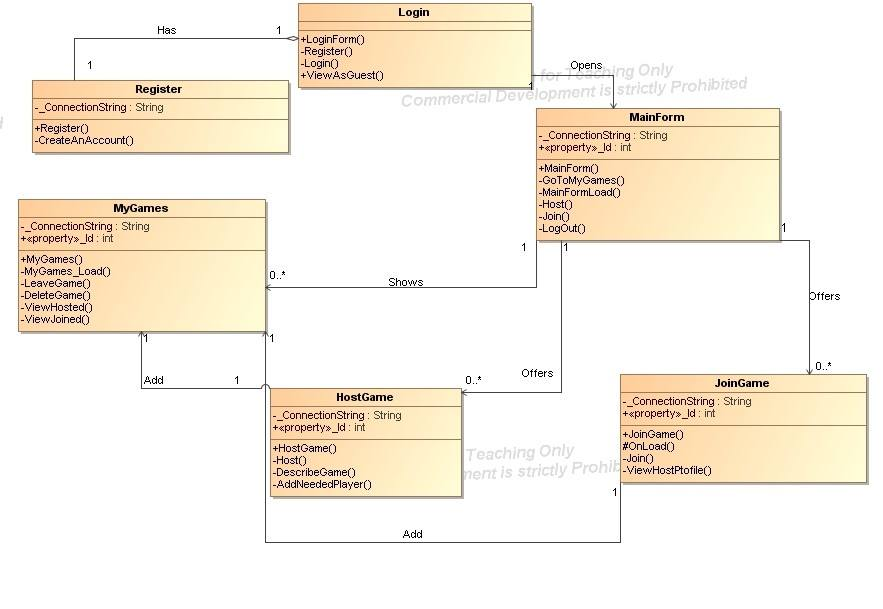
\includegraphics[scale=0.5]{img/BoardGamesClassDiagram}
				\caption{Klasių diagrama: registracija ir pgr funkcijos}
				\label{img:BoardGamesClassDiagram}
			\end{figure}
			Klasė Login, atsakinga už vartotojo autentifikaciją, turi  registracjos langą (klasę Register). Viena Login klasė gali turėti vieną   registracijos klasę. Užsiregistravus, Login klasė gali atidaryti pagrindinį vartotojo puslapį (MainForm klasę), kuris gali parodyti MyGames klasę, t.y. vartotojo žaidimus , siūlo sukurti žaidimą (HostGame) arba jungtis prie jau egzistuojančio (JoinGame) žaidimo. Kiekviena MainForm klasė gali parodyti, sukurti ir prisijungti prie kiek norimai daug žaidimų. Kiekvieną kartą sukūrus ar prisijungus prie žaidimo, jis yra pridedamas prie MyGames. 
		\subsubsection*{Antroji klasių diagramos dalis :}
			\begin{figure}[H]
				\centering
				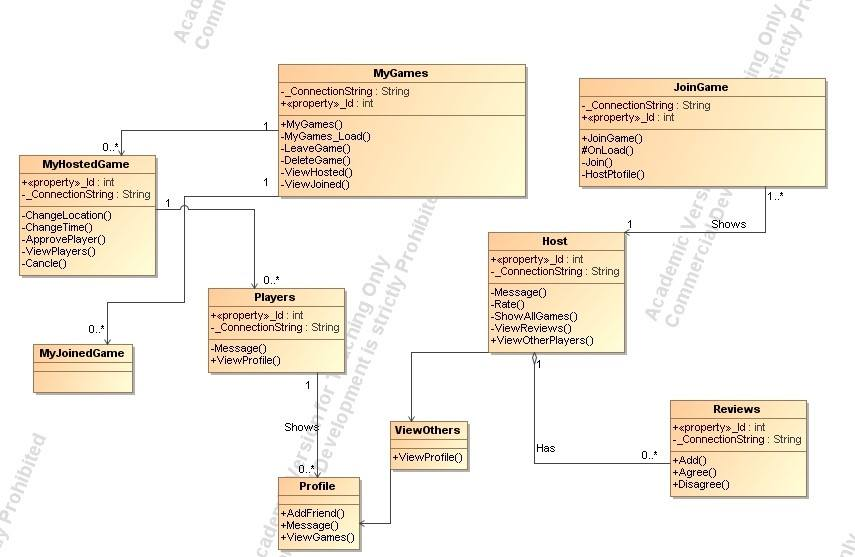
\includegraphics[scale=0.5]{img/BoardGamesClassDiagrampt1}
				\caption{Klasių diagrama: žaidimų kūrimas ir prisijungimas}
				\label{img:BoardGamesClassDiagrampt1}
			\end{figure}
			Klasė MyGames atveria vartotojo sukurtus žaidimus (klasė MyHostedGame) bei žaidimus, prie kurių jis prisijungė (MyJoinedGame). Abiejų variantų vartotojas gali turėti kiek norimai daug. Kiekvienas sukurtas žaidimas gali atverti prisijungusių kitų žaidėjų sąrašą ir iš jo yra pasiekiamas kiekvieno žaidėjo profilis (klasė Profile). Jei vartotojas pasirinko prisijungti prie žaidimo, už tai yra atsakinga JoinGame klasė, kurios vieną ar daugiau elementų (žaidimų) sukūrė konkretus kūrėjas (klasė Host). Host turi klasę Reviews, nes kiekvienas kūrėjas gali turėti atsiliepimų. Prisijungus prie žaidimo, klasė ViewOthers užtikrina galimybę peržvelgti kitų prisijungusių žaidėjų sąrašą ir jų profilius (Profile).
		\subsubsection*{Trečioji klasių diagramos dalis :}
			\begin{figure}[H]
				\centering
				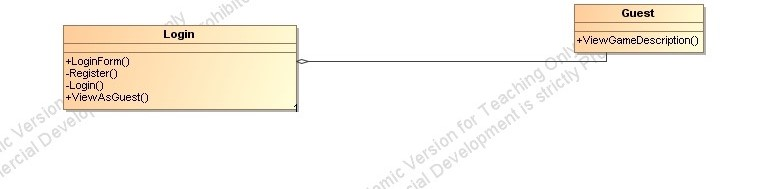
\includegraphics[scale=0.5]{img/BoardGamesClassDiagrampt2}
				\caption{Klasių diagrama: Svečias}
				\label{img:BoardGamesClassDiagrampt2}
			\end{figure}
			Jei vartotojas nėra prisiregistravęs (Guest), Login forma gali nuvesti jį prie sukurtų žaidimų sąrašo.
		\subsubsection*{Pilna klasių diagrama :}
			\begin{figure}[H]
				\centering
				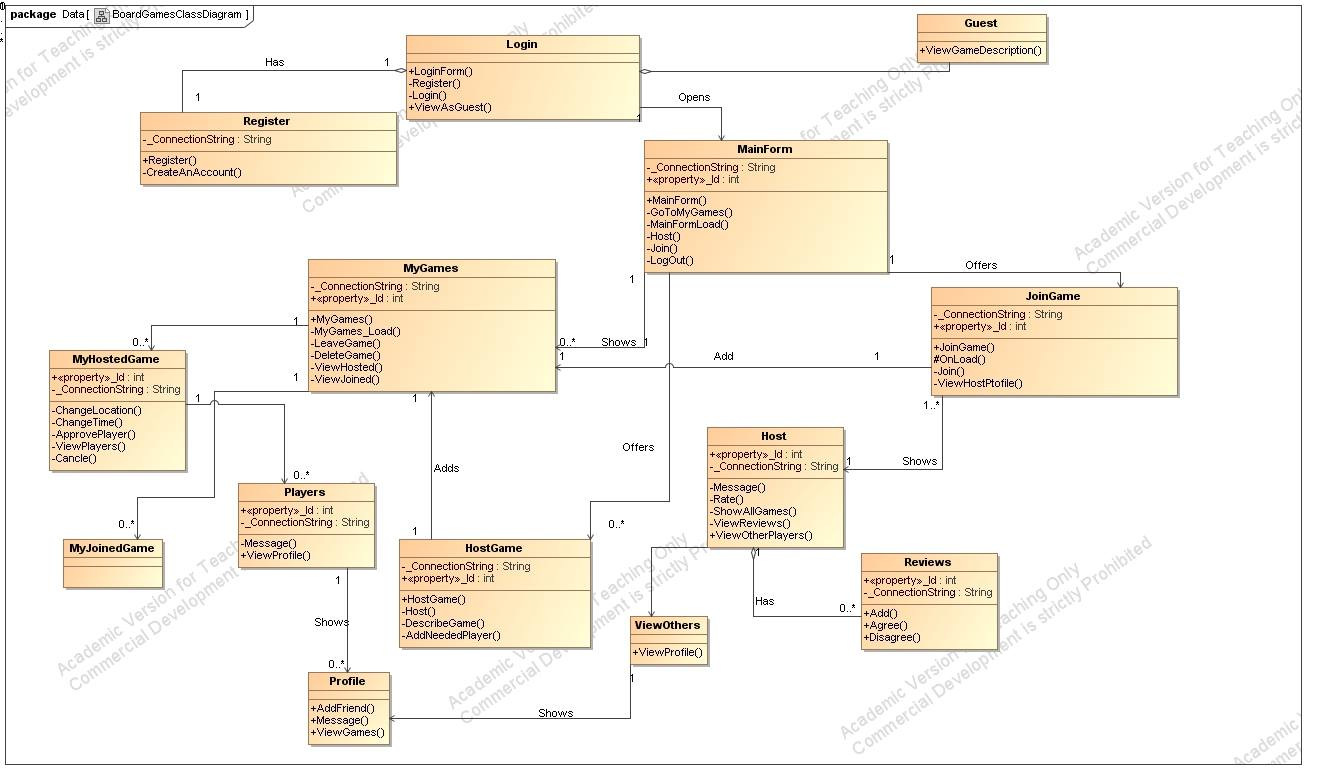
\includegraphics[scale=0.4]{img/BoardGamesClassDiagramFull}
				\caption{Visa klasių diagrama}
				\label{img:BoardGamesClassDiagramFull}
			\end{figure}
	\subsection{Objektų diagrama}
		\begin{figure}[H]
				\centering
				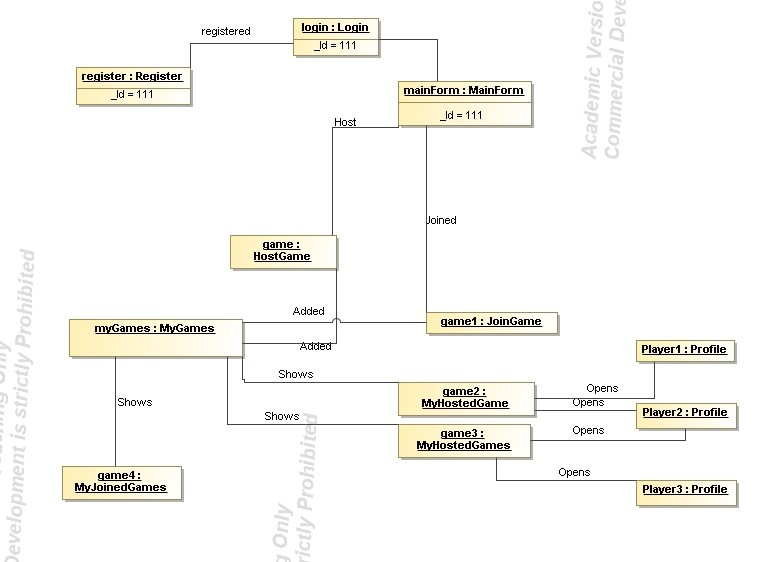
\includegraphics[scale=0.5]{img/Object}
				\caption{Objektų diagrama}
				\label{img:Object}
			\end{figure}
		Užsiregistravęs vartotojas yra autentifikuojamas ir nusiunčiamas į savo pagrindinį puslapį mainForm. Jis buvo sukūręs žaidimą game ir prisijungęs prie žaidimo game1, kurie abu buvo pridėti prie jo asmeninių žaidimų sarašo myGames. Jame jau yra žaidimai game2 ir game3 (kuriuos jis sukūrė pats) bei game4, prie kurio buvo prisijungęs. Kitas vartotojas player1 buvo prisijungęs prie žaidimo game2, player2 - prie game2 ir game3, o player3 - prie game3.

\section{Užduotys}
Pagrindinės sistemos užduotys ir su jomis susiję agentai

	\renewcommand{\labelitemi}{$\bullet$}
	\renewcommand{\labelitemii}{$\circ$}
	\begin{itemize}
		\item Agentai:
			\begin{description}
				\item [$\circ$ Svečias] Neprisijungęs programėlės naudotojas.
				\item [$\circ$ Registruotas vartotojas] Žmogus, sėkmingai atlikęs registraciją ir prisijungęs prie programėlės, galintis dalyvauti jos veikloje.
				\item [$\circ$ Žaidimo dalyvis] Registruotas vartotojas, nusprendęs prisijungti prie vieno iš sistemos siūlomų žaidimų.
				\item [$\circ$ Žaidimo šeimininkas] Registruotas vartotojas, pridėjęs žaidimą sistemoje.
				\item [$\circ$ Administratorius] Žmogus, atsakingas už tinkamą sistemos darbo palaikymą.
			\end{description}
	\end{itemize}
		
	\subsubsection*{Pagrindinės užduotys}
	
	\subsection{Svečio ir registruoto vartotojo užduotys}
		\begin{figure}[H]
			\centering
			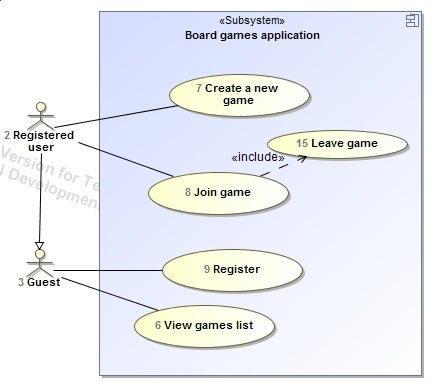
\includegraphics[scale=0.6]{img/UzduociuDiagrama1}
			\caption{Svečio ir registruoto vartotojo užduotys}
			\label{img:UzduociuDiagrama1}
		\end{figure}
		Kol vartotojas nėra užsiregistravęs sistemoje, jam suteikiamos svečio teisės, kurios leidžia tik peržiūrėti sukurtus žaidimus. Norėdamas įgyti daugiau privilegijų, vartotojas privalo užsiregistruoti. Registruotas vartotojas jau gali dalyvauti programėlės veikloje: sukurti naują žaidimą ir apie jį paskelbti, arba prisijungti prie jau esamo.

	\subsection{Žaidimo dalyvio ir šeimininko užduotys}
		\begin{figure}[H]
			\centering
			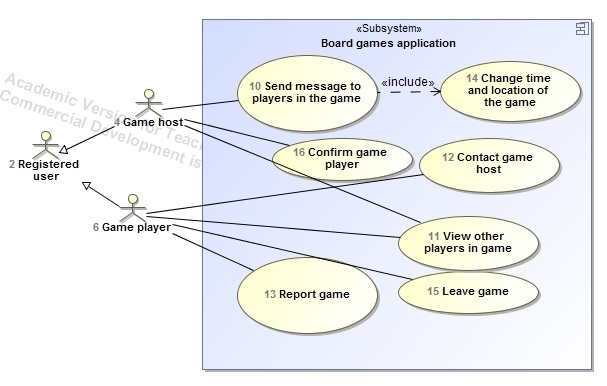
\includegraphics[scale=0.5]{img/UzduociuDiagrama2}
			\caption{Žaidimo dalyvio ir šeimininko užduotys}
			\label{img:UzduociuDiagrama2}
		\end{figure}
		Registruotas vartotojas gali atlikti du vaidmenis: arba būti sukurto žaidimo šeimininku, arba paprasčiausiu dalyviu. Žaidimo dalyviui leidžiama pranešti sistemos administratoriui apie nevykstantį žaidimą, tuo atveju, jeigu žaidėjas nuvyko į sutartą žaidimo vietą reikiamu laiku ir jam nepavyko surasti kitų užsiregistravusių dalyvių. Jeigu bent vienas žaidėjas (išskyrus šeimininką) nesutinka su tokia informacija, pranešimas laikomas melagingu. Priešingu atveju, sulaukus administratoriaus pritarimo, žaidimas išimamas iš aktyvių žaidimų sąrašo norint užkirsti tolimesnį galimą dalyvių pritraukimą. Tai pat, šeimininkui patvirtinus žaidėją, jis įgauna teisę peržiūrėti kitų, jau pareiškusių norą dalyvauti žaidėjų profilius ir su jais susipažinti naudojantis programėlės asmeninių žinučių sistema. Norėdamas pasiteirauti dėl žaidimo detalių arba visais kitais iškilusiais klausimais, jis taip pat gali tiesiogiai kreiptis į žaidimo šeimininką. Šeimininkas gali informuoti žaidėjus apie nenumatytai pasikeitusią žaidimo vietą ar laiką, susisiekti su jais ir iš anksto trumpai supažindinti su žaidimo taisyklėmis. Jeigu žaidimo dalyviui nepatinka kitų dalyvių kompanija ar bet kokios kitos žaidimo detalės, jis gali bet kada palikti žaidimą, o žaidimo šeimininkas apie tai yra informuojamas.

	\subsection{Sistemos administravimas}
		\begin{figure}[H]
			\centering
			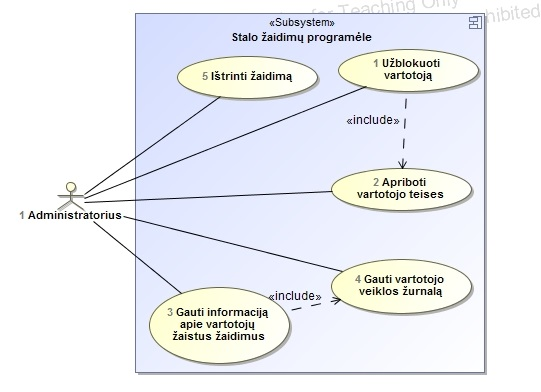
\includegraphics[scale=0.6]{img/UzduociuDiagrama3}
			\caption{Sistemos administravimas}
			\label{img:UzduociuDiagrama3}
		\end{figure}
		Administratorius prižiūri programėlės pateikiamos informacijos patikimumą. Jis turi teisę ištrinti registruoto vartotojo sukurtą žaidimą siekdamas apsaugoti dar vėliau prie žaidimo galimai prisijungsiančius dalyvius tuo atveju, jei vartotojo pateikti duomenys nėra tikslūs ar apie žaidimą jau buvo gautas įspėjamas pranešimas iš kitų sąžiningų vartotojų. Jeigu vartotojas nesiliauja kurti fiktyvių žaidimų, jam gali būti taikomos nuobaudos: laikinai (pvz. parai) apribojimas organizuoti bet kokius žaidimus. Jei tai kartojasi, administratorius gali apsvarstyti pasiūlymą užblokuoti vartotojo paskyrą ir įtraukti jį į nepageidaujamų sąrašą. Kaip pagalbinę priemonę vartotojų veiksmams sekti administratorius gali naudoti vartotojų veiklos žurnalą, kuriame būtų pateikiami chronologiškai surikiuoti vartotojų veiksmai, gauti nurodžius dominantį periodą. Veiklos žurnalą būtų galima filtruoti pagal konkretų vartotoją, taip susiaurinant paiešką.		

\section{Kūrimo pjūvis}
Komponentų dekompozicija įgyvendinta taip: nuo bendresnių komponentų pereinanama iki detalesnių.

	\subsection{Bendroji UML diagrama}
		\begin{figure}[H]
			\centering
			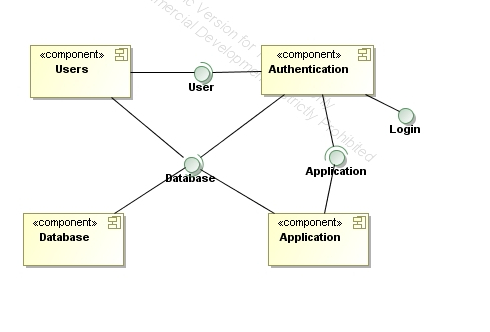
\includegraphics[scale=0.6]{img/UMLComponent1}
			\caption{Bendroji UML diagrama}
			\label{img:UMLComponent1}
		\end{figure}
		Vartotojui įsijungus stalo žaidimų aplikaciją, jis prie jos turi prisijungti, kad būtų patvirtinta jo tapatybė. Tai atliekama prisijungimo sąsajoj, kurią suteikia autentifikacijos komponentas. Patikrinus duomenis duomenų sistemoje, kurioje saugoma informacija apie vartotoją bei jo įvertinimą, gautą iš kitų žaidėjų, ir sėkmingai autentifikavus vartotoją, jam leidžiama naudotis stalo žaidimų aplikacijos ir naudotojo komponentų teikiamomis funkcijomis. Naudotojo komponento teikiama sąsaja leidžia pateikti informaciją apie save kitiems, o aplikacijos komponento sąsaja suteikia galimybę kurti žaidimus, prisijungti prie jų, vertinti vartotojus, pateikti informaciją apie esančius žaidimus pačiam vartotojui ar pačio kuriamus kitiems vartotojams.
		
		\subsection{Vartotojo komponentų diagrama}
		Aukščiau pateikta UML diagrama, kurioje vaizduojami bendri komponentai. Atskirus sistemos komponentus patogiau vaizduoti atskirai, todėl tam sukurtos papildomos diagramos.
		
		\begin{figure}[H]
			\centering
			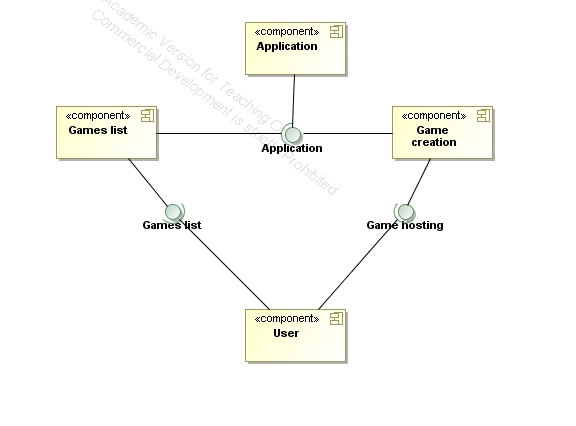
\includegraphics[scale=0.6]{img/UMLComponent2}
			\caption{Vartotojo komponentų diagrama}
			\label{img:UMLComponent2}
		\end{figure}
		Vartotojui pateikiama atitinkama sąsaja priklausomai nuo to, ar vartotojas pasirinko būti žaidimo kūrėju, ar prisijungti prie žaidimo. Jei vartotojas pasirinko prisijungti prie esamo žaidimo, tai jam yra pateikiama žaidimų sąrašo sąsaja, pateikianti sąrašą žaidimų, kuriuose trūksta narių. Jei vartotojas nusprendė pats kurti žaidimą, tada jis nukeliamas į žaidimo kūrimo langą ir įgauna papildomų funkcijų. Tai suteikia žaidimo kūrimo komponentas ir jo suteikiama žaidimo organizavimo sąsaja. Pasirinkimą būti žaidimo kurėju ar paprastu nariu bet kada galima pakeisti. 
		
		\subsection{Detalesnė vartotojo komponentų diagrama}
		Kadangi vartotojai gali arba prisijungti prie žaidimų, arba būti jų kūrėjais, jiems reikalingi atitinkami komponentai. Kad geriau matytųsi, kokie iš jų priklauso kiekvienam tipui, sukurta atskira UML diagrama.
		
		\begin{figure}[H]
			\centering
			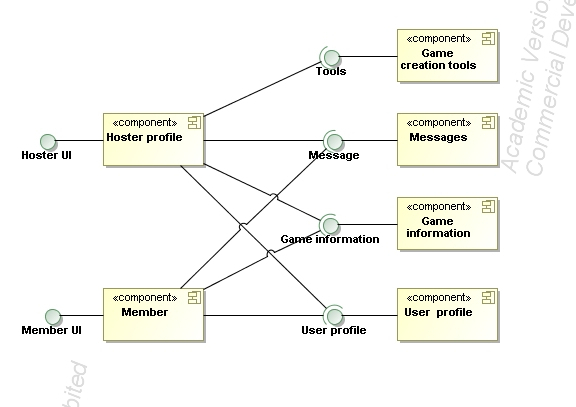
\includegraphics[scale=0.6]{img/UMLComponent3}
			\caption{Detalesnė vartotojo komponentų diagrama}
			\label{img:UMLComponent3}
		\end{figure}
		Tiek paprasti nariai, tiek kūrėjai gali naudotis vartotojo profilio, žaidimo informacijos ir žinučių komponentais, kurie suteikia atitinkamas sąsajas. Vartotojo profilio komponentas leidžia parodyti informaciją apie žaidimuose esančius narius bei jų įvertinimą ir patikimumą. Žaidimo informacijos komponente trumpai nupasakojama apie žaidimą bei pateikiamas jo pavadinimas. Žinučių komponentas suteikia galimybę susisiekti su kiekvienu žaidimo nariu atskirai ir bendrauti bendrame grupės pokalbyje. Kūrėjas taip pat gali naudotis žaidimo kūrimo įrankių komponentu. Jam suteikiamos galimybės pateikti ir keisti žaidimo informaciją, priimti, pakviesti bei išmesti žaidimo narius.

\section{Fizinis pjūvis}
Šioje dalyje pateikta informacija apie sistemos fizinius mazgus, juose įdiegtas vykdomasias aplinkas, reikalingas vykdyti programos komponentų darbą, taip pat apie komunikaciją tarp mazgų ir juose įdiegtus artifaktus, kurie saugo programinį kodą.
	\subsection{Fiziniai mazgai tinkle, jų komunikacija}
				\begin{figure}[H]
				\centering
				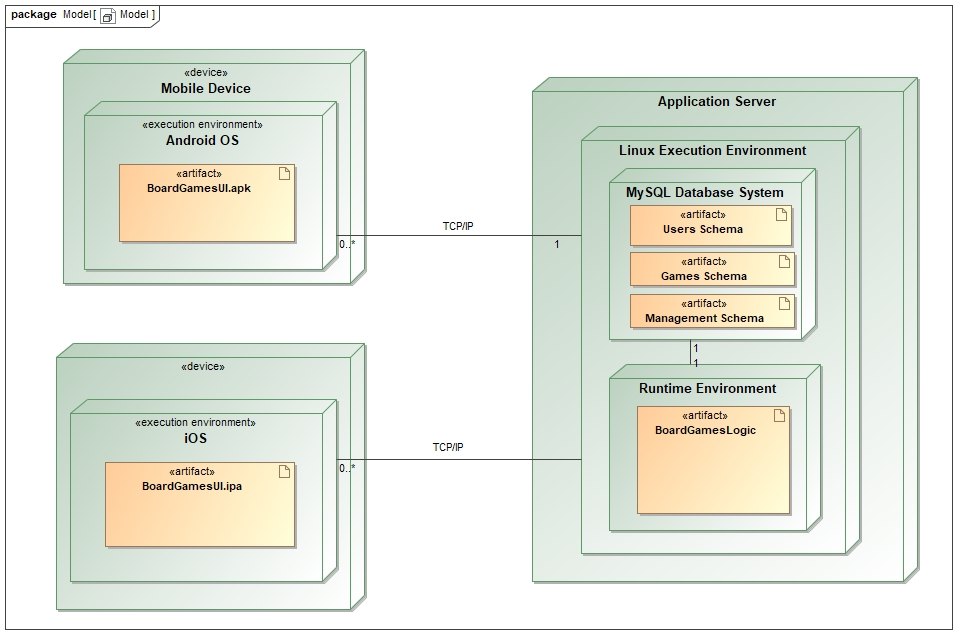
\includegraphics[scale=0.5]{img/NodesCommunication}
				\caption{Fizinių sistemos mazgų išdėstymo tinkle diagrama}
				\label{img:NodesCommunication}
			\end{figure}
			Mobilioji aplikacija dėl savo paprasto loginio pobūdžio nereikalauja 				kompleksiškos tinklo architektūros su daugybe fizinių komponentų. 				Išdėstymo diagramoje pateiktas kliento mazgas – mobilusis įrenginys – 				kuriame veikia Android OS arba iOS. Šiose operacinių sistemų aplinkose 				diegiamas mobiliosios aplikacijos artifaktas (.apk – Android atveju, .ipa 				– iOS atveju), kurį sudaro visos sukompiliuotos projekto vartotojo sąsajos 				klasės, resursai, taip pat ir nesukompiliuoti resursai. Kitas mazgas – 				nutolęs aplikacijos serveris, su kuriuo TCP/IP protokolu komunikuoja kliento mobilusis įrenginys. Šiame nutolusiame fiziniame serveryje veikia stabili Linux OS 				aplinkos distribucija, užtikrinanti duombazės pasiekiamumą ir darbo 				nepertraukiamumą. Šioje OS instaliuota MySQL duomenų bazių valdymo 				sistema, kurioje sukurtos trys lentelių schemos: Users (informacija, 				susijusi su aplikacijos naudotojais), Games (informacija, susijusi su 				žaidimais, jų sesijomis), Management (aplikacijos valdymo, statistinių 				duomenų schema). Taip pat šioje Linux aplinkoje veikia programėlės loginio 				kodo vykdomoji aplinka, kurioje įdiegtas loginis artifaktas, atsakingas už 				visą programėlės logiką.
	\subsection{Artifaktų diegimas į mazgus}
				\begin{figure}[H]
				\centering
				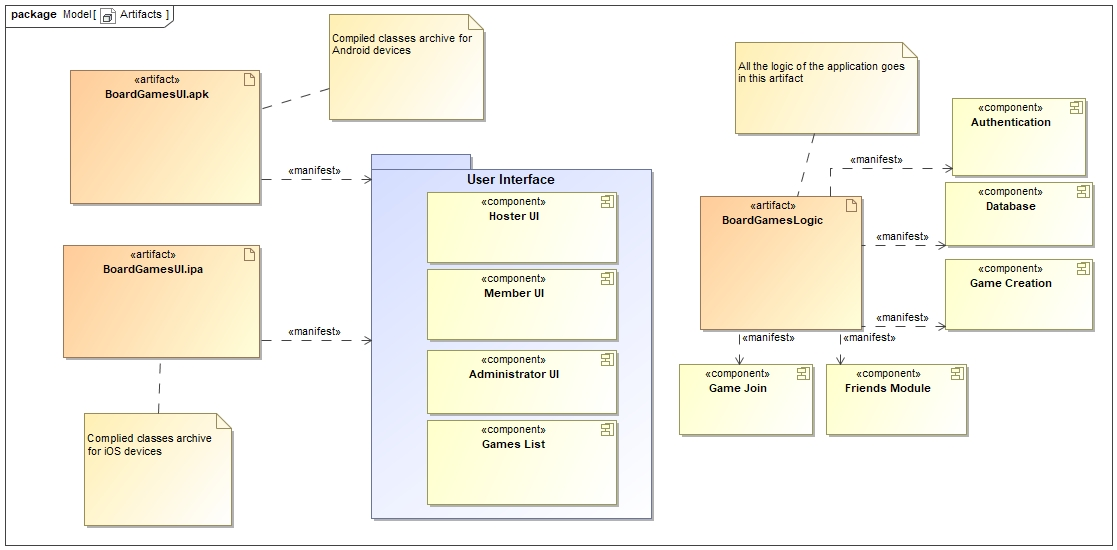
\includegraphics[scale=0.4]{img/Artifacts}
				\caption{Artifaktų sandara ir diegimas į mazgus}
				\label{img:Artifacts}
			\end{figure}
			Sistemą sudaro du pagrindiniai artifaktai - įdiegtas vartotojo sąsajos 				paketas, išdėstomas kliento mobiliajame įrenginyje, ir logikos paketas, 			įdiegtas nutolusio aplikacijos serverio kodo vykdomojoje aplinkoje. 
		\subsubsubsection*{Mobiliajame įrenginyje įdiegto artifakto turinys:}
  				\begin{itemize}
					\item Žaidimo šeimininko vartotojo sąsajos komponentas
					\item Paprasto programėlės naudotojo vartotojo sąsajos komponentas.
					\item Administratoriaus vartotojo sąsajos komponentas
					\item Esamų žaidimų sąrašas ir informacija apie juos
				\end{itemize}
		\subsubsubsection*{Nutolusiame serveryje įdiegto artifakto turinys:}
  				\begin{itemize}
					\item Autentifikacijos komponentas - visa logika, susijusi 						su prisijungimu, registracija 
					\item Duombazės komponentas - logika, kurioje apibrėžta 					komunikacija su DBVS
					\item Žaidimo sukūrimo logika - validacija, patvirtinimas, 
					sistemos informavimas
					\item Prisijungimo prie žaidimo logika - validacija, 						žaidimo šeimininko, kitų žaidėjų informavimas 
					\item Draugų modulio komponentas - visa logika, 					apibrėžianti galimą tarpusavio komunikaciją tarp 						programėlės naudotojų
				\end{itemize}
			Taip pat nutolusiame serveryje veikiančios Duomenų bazės valdymo 				sistemos aplinkoje įdiegti šie artifaktai, apibrėžiantys loginį 			duomenų bazės lentelių išskaidymą:
  				\begin{itemize}
					\item Naudotojų lentelių schema
					\item Žaidimų lentelių schema
					\item Valdymo, priežiūros lentelių schema
				\end{itemize}
	\subsection{Topologinio išdėstymo tinkle pavyzdys}
				\begin{figure}[H]
				\centering
				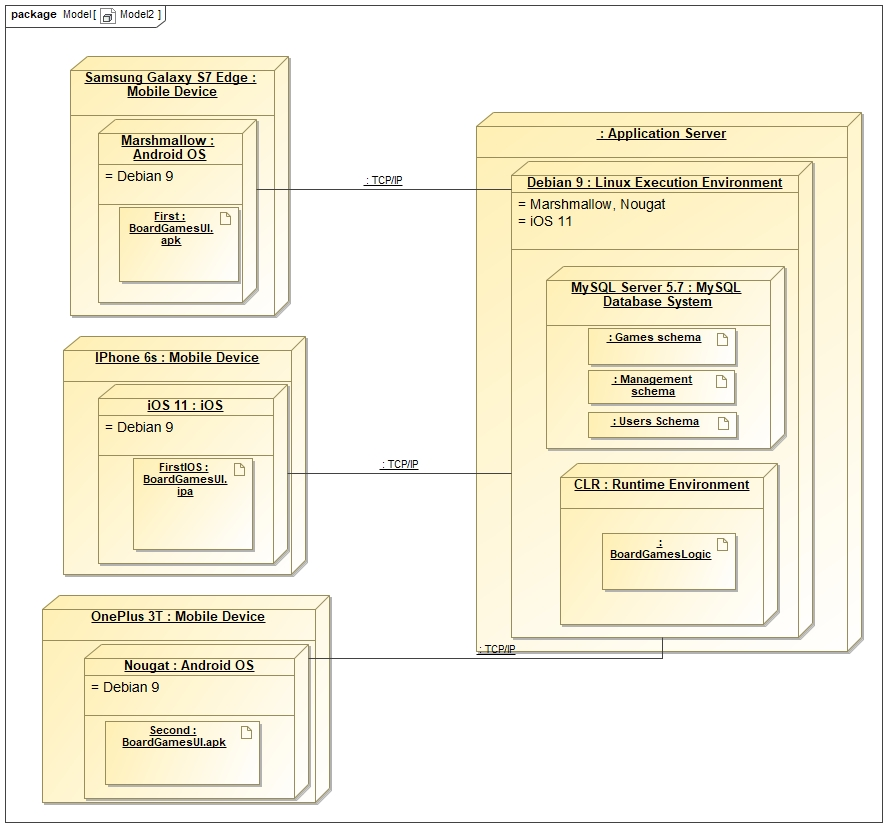
\includegraphics[scale=0.4]{img/TopologyExample}
				\caption{Fizinio išdėstymo tinkle pavyzdys, komunikacija}
				\label{img:TopologyExample}
			\end{figure}
		Diagramoje pavaizduotas galimas realaus sistemos vaizdo atvejis, kuris atitinka 		anksčiau aprašytą mazgų komunikacijos ir artifaktų diegimo logiką. Pavyzdyje 			pateikti trys klientiniai įrenginiai (2 Android, 1 iOS), kurie TCP/IP protokolo 		pagalba komunikuoja su konkrečiu Linux Debian 9.0 distribucijos serveriu, kuriame 			įdiegtas MySQL 5.7 versijos serveris, apdorojantis programėlės SQL užklausas ir 		Common Language Runtime vykdomoji aplinka, apdorojanti loginį programinį kodą, jį 			paverčianti mašininiu, kurį vėliau įvykdo fizinis mazgas.
			
\section{Procesų pjūvis}
Aplikacijoje yra vartotojo sąsajos, duomenų apdorojimo ir duomenu bazės procesai. 
Vartotojas tiesiogiai bendraudamas su vartotojo sąsaja, siunčia asinchronines 
žinutes duomenų apdorojimo procesui, kuris savo ruožtu bendrauja su duomenų baze.

	\subsection{Prisijungimas}
		\subsubsection*{Prisijungimo procesų sekos diagrama :}
		\begin{figure}[H]
			\centering
			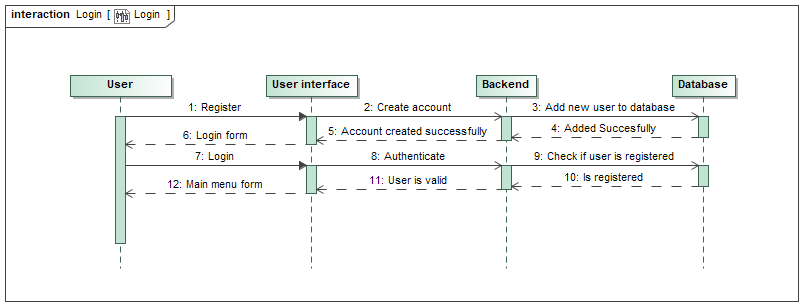
\includegraphics[scale=0.5]{img/Login_sequence}
			\caption{Prisijungimo procesų sekų diagrama}
			\label{img:MainWindow_activity}
		\end{figure}
		Visų pirma vartotojas privalo užsiregistruoti. Vartojo sąsaja nusiunčia JSON 
		žinutę su gautais duomenimis loginiam procesui, kuris patikrina ar duomenys yra tinkami ir
		prideda vartotoją į duomenų bazę. Užsiregistravęs vartotojas turi prisijungti,
		procedūra ganėtinai panaši - vartotojo sąsajoje gauti duomenys patikrinami ir 
		jei jie yra validūs, patikrinama ar slaptažodis sutampa su esančiu duomenų
		bazėje. Autentifikuotas vartotojas yra prijungiamas prie programėlės. 
		Jei slaptažodis netinka arba vartotojas nerastas duomenų bazėje, leidžiama
		patikslinti prisijungimo laukus ir prisijungimo procesas kartojamas dar kartą.
		\subsubsection*{Prisijungimo/Registracijos procesų veiklos diagrama :}
		\begin{figure}[H]
			\centering
			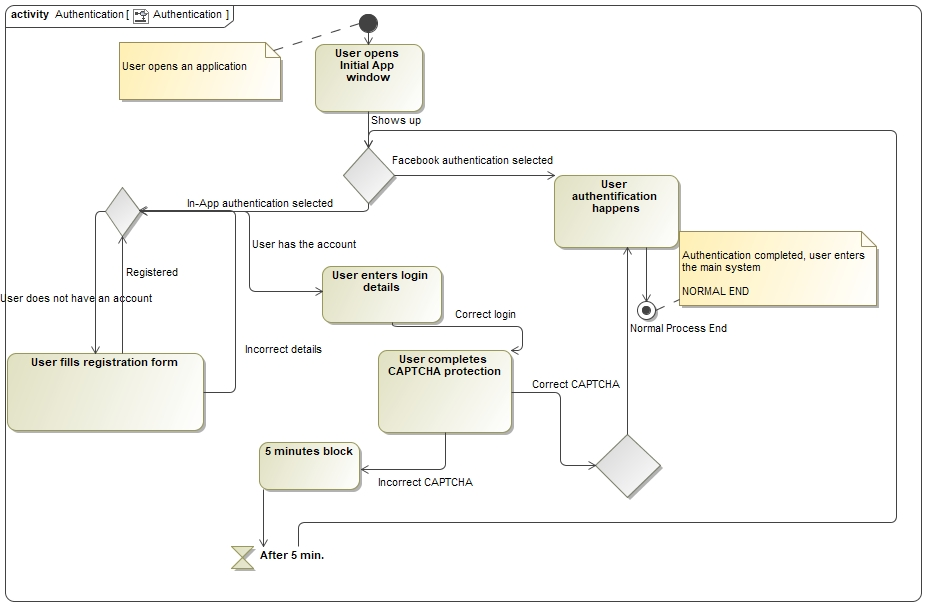
\includegraphics[scale=0.5]{img/Authentication}
			\caption{Autentifikacijos veiklos diagrama}
			\label{img:Authentication}
		\end{figure}
		Kiekvienas programėlės naudotojas patenka į prisijungimo langą, kuriame gali 			pasirinkti vieną iš galimų prisijungimo būdų - naudojantis Facebook API arba 			paprasta vartotojo paskyra. Pasirinkus Facebook autentifikacija, programėlė 			nuskaito vartotojo identifikacinius duomenis ir ši veikla pabaigiama. Pasirinkus 			prisijungimą naudojantis paprasta paskyra atsiranda dvi galimybės - prisijungti 		arba užsiregistruoti. Pasirinkus registraciją vartotojas suveda savo duomenis, 			jeigu pastarieji teisingi - jis užregistruojamas ir gali prisijungti. Jei duomenys 			klaidingi - vartotojas vėl patenka į tą patį registracijos langą. Norėdamas 			prisijungti vartotojas turi įvesti savo teisingus prisijungimo duomenis, tuomet 		iššoka CAPTCHA patvirtinimo paveikslėlis, skirtas prevencijai nuo kenkėjiško tipo 			skriptų ir programų, imituojančių žmogų. Jeigu CAPTCHA klaidingas - vartotojas 			blokuojamas 5 minutėms (tiek laiko negali prisijungti siekiant taupyti sistemos 		resursus, išvengti DOS/DDOS atakų). Suvedus teisingą CAPTCHA kodą patenkama į 			sistemą ir ši veikla užbaigiama.
	\subsection{Pagrindinis navigacijos langas}
		\begin{figure}[H]
			\centering
			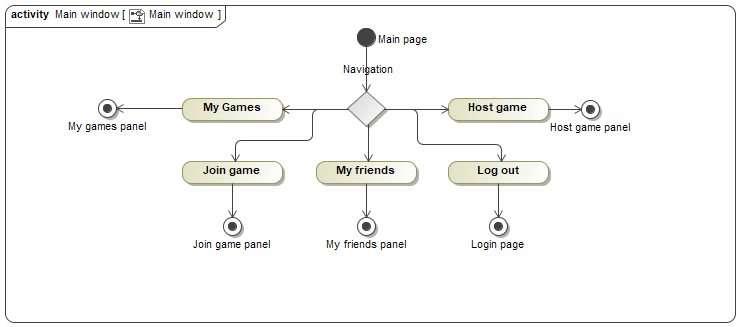
\includegraphics[scale=0.5]{img/MainWindow_activity}
			\caption{Pagrindinio navigacijos lango veiklos diagrama}
			\label{img:MainWindow_activity}
		\end{figure}
		\subsubsection*{Pagrindiniame navigacijos lange vartotojas paspaudęs atitinkamus mygtukus gali:}
			\renewcommand{\labelitemi}{$\bullet$}
			\begin{itemize}
				\item Atidaryti žaidimo sukūrimo langą.
				\item Atidaryti prisijungimo prie žaidimo langą.
				\item Atidaryti draugų sąrašo langą.
				\item Atidaryti mano žaidimų langą
				\item Atsijungti
			\end{itemize}

	\subsection{Žaidimo sukūrimo langas}
		\subsubsection*{Žaidimo sukūrimo veiklos diagrama :}
			\begin{figure}[H]
				\centering
				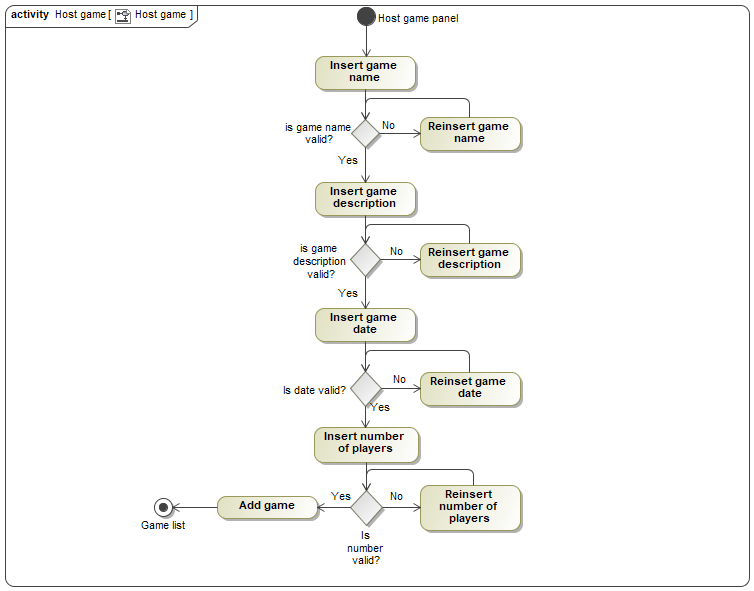
\includegraphics[scale=0.5]{img/HostGame_activity}
				\caption{Žaidimo sukūrimo veiklos diagrama}
				\label{img:Hostgame_activity}
			\end{figure}
			\subsubsubsection*{Žaidimo sukūrimo lange vartotojas turi įvesti :}
				\renewcommand{\labelitemi}{$\bullet$}
				\begin{itemize}
					\item Žaidimo pavadinimą.
					\item Žaidimo aprašymą.
					\item Žaidimo datą.
					\item Žaidėjų skaičių
				\end{itemize}
			Įvedimo metu tikrinama ar duomenys įvesti leistinu formatu. Jei formatas 
			netinkamas, vartotojas turi pataisyti atitinkamus duomenų laukus. Tinkamai
			užpildžius laukus,leidžiama pridėti žaidimą.
		\subsubsection*{Žaidimo sukūrimo procesų sekų diagrama :}
			\begin{figure}[H]
				\centering
				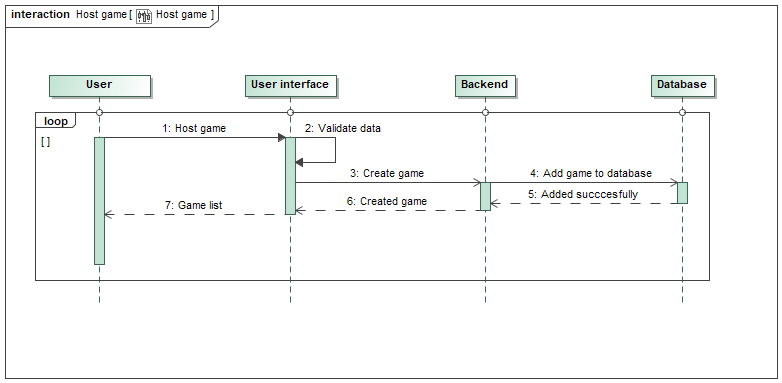
\includegraphics[scale=0.5]{img/HostGame_sequence}
				\caption{Žaidimo sukūrimo procesų sekų diagrama}
				\label{img:Hostgame_sequence}
			\end{figure}
			Vartotojas norėdamas sukurti žaidimą įveda žaidimo duomenis. Įvedimo metu 
			tikrinama ar duomenys įvesti leistinu formatu. Jei duomenys tinkami, tada 
			jie JSON formatu išsiunčiami loginiam procesui, kuris sukuria žaidimą ir 
			įrašo jį į duomenų bazę.	
			
	\subsection{Prisijungimo prie egzistuojančio žaidimo langas}	
		\subsubsection*{Prisijungimo prie egzistuojančio žaidimo veiklos diagrama :}
			\begin{figure}[H]
				\centering
				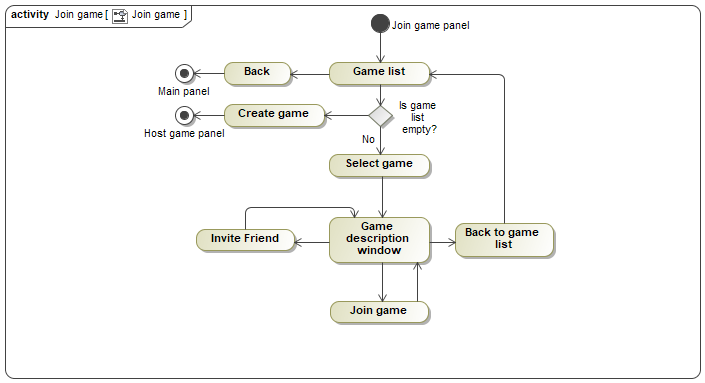
\includegraphics[scale=0.5]{img/JoinGame_activity}
				\caption{Prisijungimo prie egzistuojančio žaidimo veiklos diagrama}
				\label{img:JoinGame_activity}
			\end{figure}
			Iš pradžių vartotojui atidaromas egzistuojančių žaidimų sąrašas. Čia 
			vartotojas gali grįžti pagrindinį navigacijos langą arba tęsti žaidimo
			pasirinkimą. Jei nėra žaidimų prie kurių būtų galima prisijungti, vartotojui
			pasiūloma sukurti naują žaidimą. Vartotojui sutikus jis nukreipiamas į 
			žaidimo sukūrimo langą. Jei žaidimų sąrašas nėra tučias, tai vartotojas
			gali pasirinkti žaidimą prie kurio norėtų prisijungti. Pasirinkus atidaromas
			pasirinkto žaidimo aprašymo langas. Čia vartotojas gali pakviesti draugus
			kartu žaisti pasirinktą žaidimą, pats prisijungti prie žaidimo arba grįžti
			atgal į žaidimų sąrašą ir pasirinkti kitą žaidimą.
		\subsubsection*{Prisijungimo prie egzistuojančio žaidimo sekų diagrama :}
			\begin{figure}[H]
				\centering
				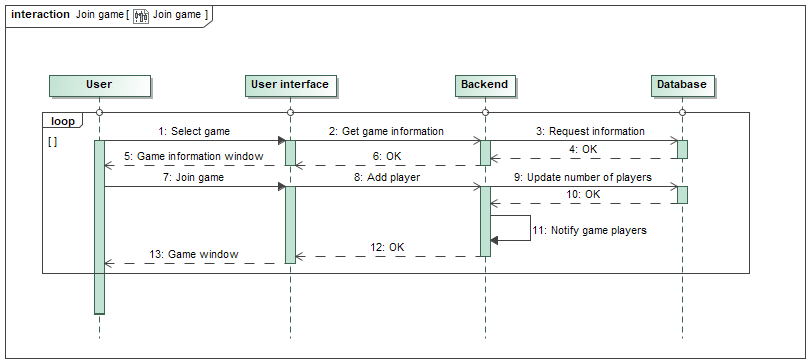
\includegraphics[scale=0.5]{img/JoinGame_sequence}
				\caption{Prisijungimo prie egzistuojančio žaidimo procesų sekų diagrama}
				\label{img:Hostgame_sequence}
			\end{figure}
			Žaidėjui pasirinkus žaidimą iš sąrašo, atidaromas žaidimo informacijos 
			langas. Informaciją apie žaidimą suteikia logikos procesas, kuris
			nusiuntęs užklausą į duomenų bazę, gauna papildomą informaciją apie 
			pasirinktą žaidimą. Vartotojui nusprendus prisijungti prie žaidimo, 
			nusiunčiama žinutė atnaujinti prisijungusių žaidėjų skaičių duomenų bazėje,
			taip pat visiems tame žaidime užsiregistravusiems žaidėjams išsiunčiamas 
			pranešimas apie naują prisijungusį žaidėją.

	\subsection{Draugų sąrašo langas}		
		\subsubsection*{Draugų sarašo lango sekų diagrama :}
			\begin{figure}[H]
				\centering
				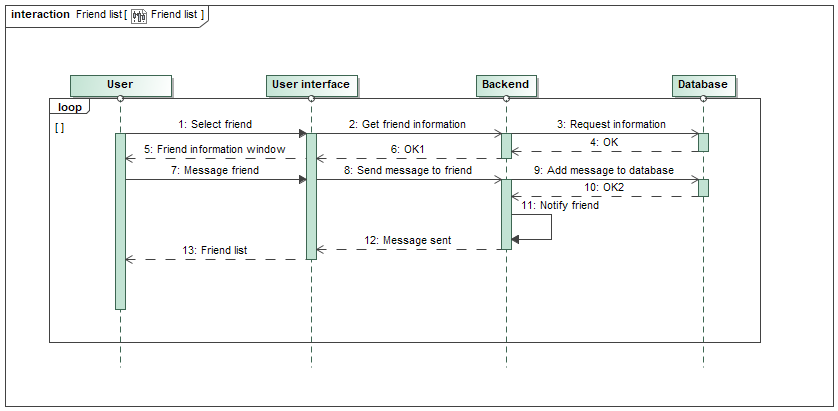
\includegraphics[scale=0.5]{img/FriendList_sequence}
				\caption{Draugų sarašo lango sekų diagrama}
				\label{img:FriendList_sequence}
			\end{figure}
			Vartotojui pasirinkus draugą iš draugų sąrašo, paprašoma loginio proceso
			gauti daugiau duomenų apie draugą iš duomenų bazės. Tuomet atidaromas 
			langas su daugiau duomenų apie draugą. Paspaudus siųsti žinutę logikos 
			procesas išsaugo žinutę duomenų bazėje ir praneša draugui apie gautą žinutę.
			
	\subsection{Žaidimo langas}		
		\subsubsection*{Žaidimo lango sekų diagrama :}
			\begin{figure}[H]
				\centering
				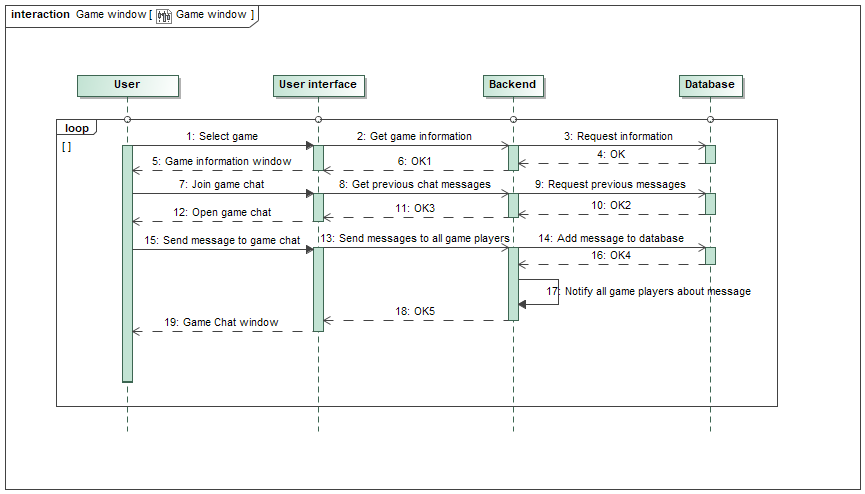
\includegraphics[scale=0.5]{img/GameWindow_sequence}
				\caption{Žaidimo lango sekų diagrama}
				\label{img:GameWindow_sequence}
			\end{figure}
			Vartotojui pasirinkus žaidimą iš žaidimų sąrašo, paprašoma loginio proceso
			gauti daugiau duomenų apie žaidimą iš duomenų bazės. Tuomet atidaromas 
			langas su daugiau duomenų apie žaidimą. Paspaudus siųsti žinutę logikos 
			procesas paprašo žaidimo susirašinėjimo istorijos iš duomenų bazės. Tada
			atidaromas pokalbių langas, kur vartotojas gali išsiųsti žinutę visiems 
			prie žaidimo prisijungusiems žaidėjams. Paspaudus siųsti žinutę logikos 
			procesas išsaugo žinutę duomenų bazėje ir praneša žaidėjams apie gautą žinutę.
	
\sectionnonum{Literatūros sąrašas}
\begin{itemize}
	\item Doc. dr. K. Petrausko Programų Sistemų Inžinerijos kurso konspektai
	\item UML dokumentacija \url{https://www.tutorialspoint.com/uml/uml_2_overview.htm}
\end{itemize}
		
\end{document}
